\section{Further Analysis and Discussion}
\label{sec:analysis}

\subsection{How Many Attackers Does It Take?}
\label{sec:dose}

\begin{figure}[!t]
  \centering
  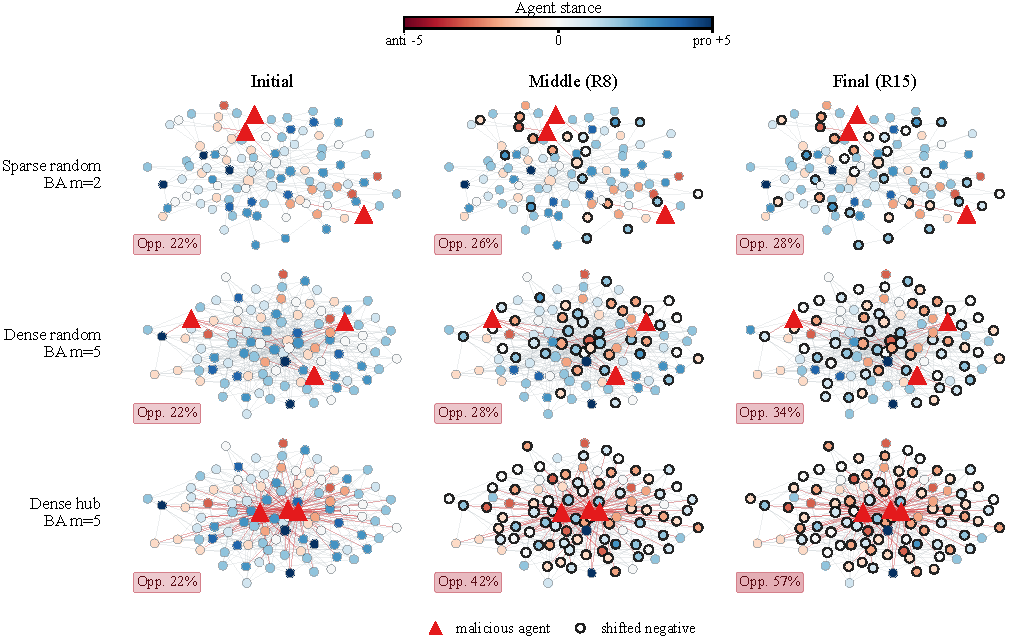
\includegraphics[width=\columnwidth]{fig_network_topology.pdf}
  \caption{Stance snapshots for three network topologies under the same Pseudo-Rational attack (Vaccine Mandate). Node colour encodes stance (warm = positive, cool = negative); stars mark opposition-shifted agents. Hub-anchored placement roughly doubles the opposition share compared to dense random placement, confirming that network position amplifies impact beyond added connectivity.}
  \label{fig:network_evo}
\end{figure}

We replicate the vaccine-mandate condition while varying the number of attackers from $n{=}3$ to $n{=}20$ on Pseudo-Rational and Victim Narrative (Table~\ref{tab:dose}). Both show clear dose--response trends in stance damage with no plateau before 20\%. Victim Narrative saturates the emotional climate from very few attackers because each negative-emotion message invites negative responses from neighbours, while Pseudo-Rational requires sustained density from more vantage points. The three-attacker setting used in our main studies therefore sits on the low end of a curve that does not flatten before the densities typical of coordinated campaigns~\citep{Ferrara2016}.

\begin{table}[!t]
\centering
\caption{Dose--response of Pseudo-Rational (PR) and Victim Narrative (VN) as attacker count $n$ increases from 3 to 20. Both strategies show a clear upward trend in stance damage ($\Delta\bar{s}$) with no plateau. \textbf{Bold} marks the peak within each strategy.}
\label{tab:dose}

\vspace{2pt}
\renewcommand{\arraystretch}{1.12}
\setlength{\tabcolsep}{2.4pt}

\scriptsize
\begin{tabular}{@{}l r rrr rr@{}}
\toprule
& & \multicolumn{3}{c}{\textit{Stance}}
& \multicolumn{2}{c}{\textit{Emotion}} \\
\cmidrule(lr){3-5}\cmidrule(l){6-7}
\textbf{Condition} & $n$
& {$\bar{s}_T$} & {$\Delta\bar{s}$} & {NSR}
& {EV} & {ENI} \\
\midrule
\rowcolor{rowalt}
\textsc{Baseline} & 0
  & $+$1.52 & $+$0.34 & 5.0
  & $+$0.28 & 36.1 \\
\midrule
\multicolumn{7}{@{}l}{\textit{Pseudo-Rational Scepticism}} \\
\quad PR & 3
  & $-$0.74 & $-$1.92 & 85.6
  & $-$0.39 & 71.2 \\
\rowcolor{rowalt}
\quad PR & 5
  & $-$1.05 & $-$2.25 & 85.3
  & $-$0.32 & 65.9 \\
\quad PR & 10
  & $-$1.64 & $-$2.81 & 91.1
  & $-$0.32 & 65.9 \\
\rowcolor{rowalt}
\quad PR & 20
  & $\mathbf{-2.05}$ & $\mathbf{-3.24}$ & $\mathbf{95.0}$
  & $\mathbf{-0.82}$ & $\mathbf{90.9}$ \\
\midrule
\multicolumn{7}{@{}l}{\textit{Victim Narrative}} \\
\quad VN & 3
  & $-$0.40 & $-$1.57 & 76.3
  & $-$0.72 & 87.0 \\
\rowcolor{rowalt}
\quad VN & 5
  & $-$0.76 & $-$1.96 & 82.1
  & $-$0.85 & 92.6 \\
\quad VN & 10
  & $-$1.52 & $-$2.69 & 87.8
  & $-$0.83 & 91.7 \\
\rowcolor{rowalt}
\quad VN & 20
  & $\mathbf{-2.00}$ & $\mathbf{-3.19}$ & $\mathbf{95.0}$
  & $\mathbf{-0.90}$ & $\mathbf{94.8}$ \\
\bottomrule
\end{tabular}
\end{table}


\subsection{Where Attackers Sit in the Network}
\label{sec:network}

We rerun the strongest Pseudo-Rational condition on a sparse random, a dense random, and a dense hub-anchored network (Figure~\ref{fig:network_evo}). The same three attackers roughly double the opposition share on the hub network compared to the dense random one. Replacing a random topology with a hub-anchored one thus adds far more damage than simply increasing average degree~\citep{GonzalezBailon2013}, and a scaling check up to $N{=}5000$ (Appendix~\ref{app:scale}) confirms that the pattern holds at the local-cluster level even in much larger populations. Rate-limiting hub-anchored coordinated activity should therefore greatly reduce the worst case without inspecting content.

\subsection{Governance Implications}
\label{sec:implications}

The main governance lesson is that narrative defence should be organised around attack mechanisms, not a generic moderation pipeline. When harm comes from moral framing, the problem is not a single false claim but an interpretive lens. Early structural inoculation helps participants recognise manipulative forms before they dominate the thread. Trust-style attacks depend on evidence and institutional credibility (Studies~1--2), so fact-checking and source transparency are natural candidates for targeted follow-ups against such strategies.

A second implication is that governance cannot focus on content alone. The same message can be damaging or harmless depending on audience composition, and a few attackers gain outsized influence near network hubs. Platforms should pair message-level responses with structural friction against coordinated amplification, especially in LLM-based communities where malicious agents may be cheap and strategically placed. Robust governance is less about judging every contested claim than about reducing the leverage that coordinated manipulation can gain.
